%!TEX root = ../thesis.tex

\chapter[Evolution of a Reliable and Extensible High-Level Control System]{Evolution of a Reliable and Extensible High-Level Control System for an Autonomous Car}
\label{ch:evo}

\ifpdf
	\graphicspath{{Chapter7/Figs/Raster/}{Chapter7/Figs/PDF/}{Chapter7/Figs/}}
\else
	\graphicspath{{Chapter7/Figs/Vector/}{Chapter7/Figs/}}
\fi

The reliability of autonomous vehicles is heavily dependent on their software frameworks, which are required to interface and process data from many different sensors on board the vehicle, perform navigational processes such as path planning and lane keeping, take action to ensure safety and display data to an operator in a useful fashion. These sensors can include a combination of cameras, LiDARs, GPS, IMU, and odometric sensors to achieve positioning and localisation for the vehicle and nearby objects in their environment and can be challenging to integrate. In this paper, we present a hybridised software framework that combines sensor and navigational processing for autonomous driving. Our framework utilises a modular approach for interfacing and safety functionality, whilst navigation and sensor interfaces are implemented as nodes in the Robot Operating System (ROS). Our testing results verify the suitability of our framework by integration with a hardware-in-the-loop simulation system and for fully autonomous field driving.

\section{Introduction}
The Renewable Energy Vehicle Project (REV) at UWA has developed an intelligent autonomous test vehicle, utilising a Formula-SAE race car (see Fig.~\ref{fig:7:car}) as a platform (Formula SAE~\cite{sae_international_student_nodate} is an annual student competition organised by the Society of Automotive Engineers with events worldwide). Using such a vehicle allows us to target driving applications, both on- and off-road, in structured and unstructured driving environments. We have incorporated full drive-by-wire control of the electric vehicle's throttle, steering and the hydraulic braking system. The use of a Formula-SAE car provides several advantages for such a project as the vehicle is mechanically simple. Formula-SAE cars with similar designs are common at universities worldwide and the size of the vehicle makes testing accessible. Furthermore, the use of an electric vehicle makes the project significantly more practical for student work and the hardware installed in this project can take advantage of the large amount of electrical energy already available on the vehicle.

\begin{figure}[H]
	\centering
	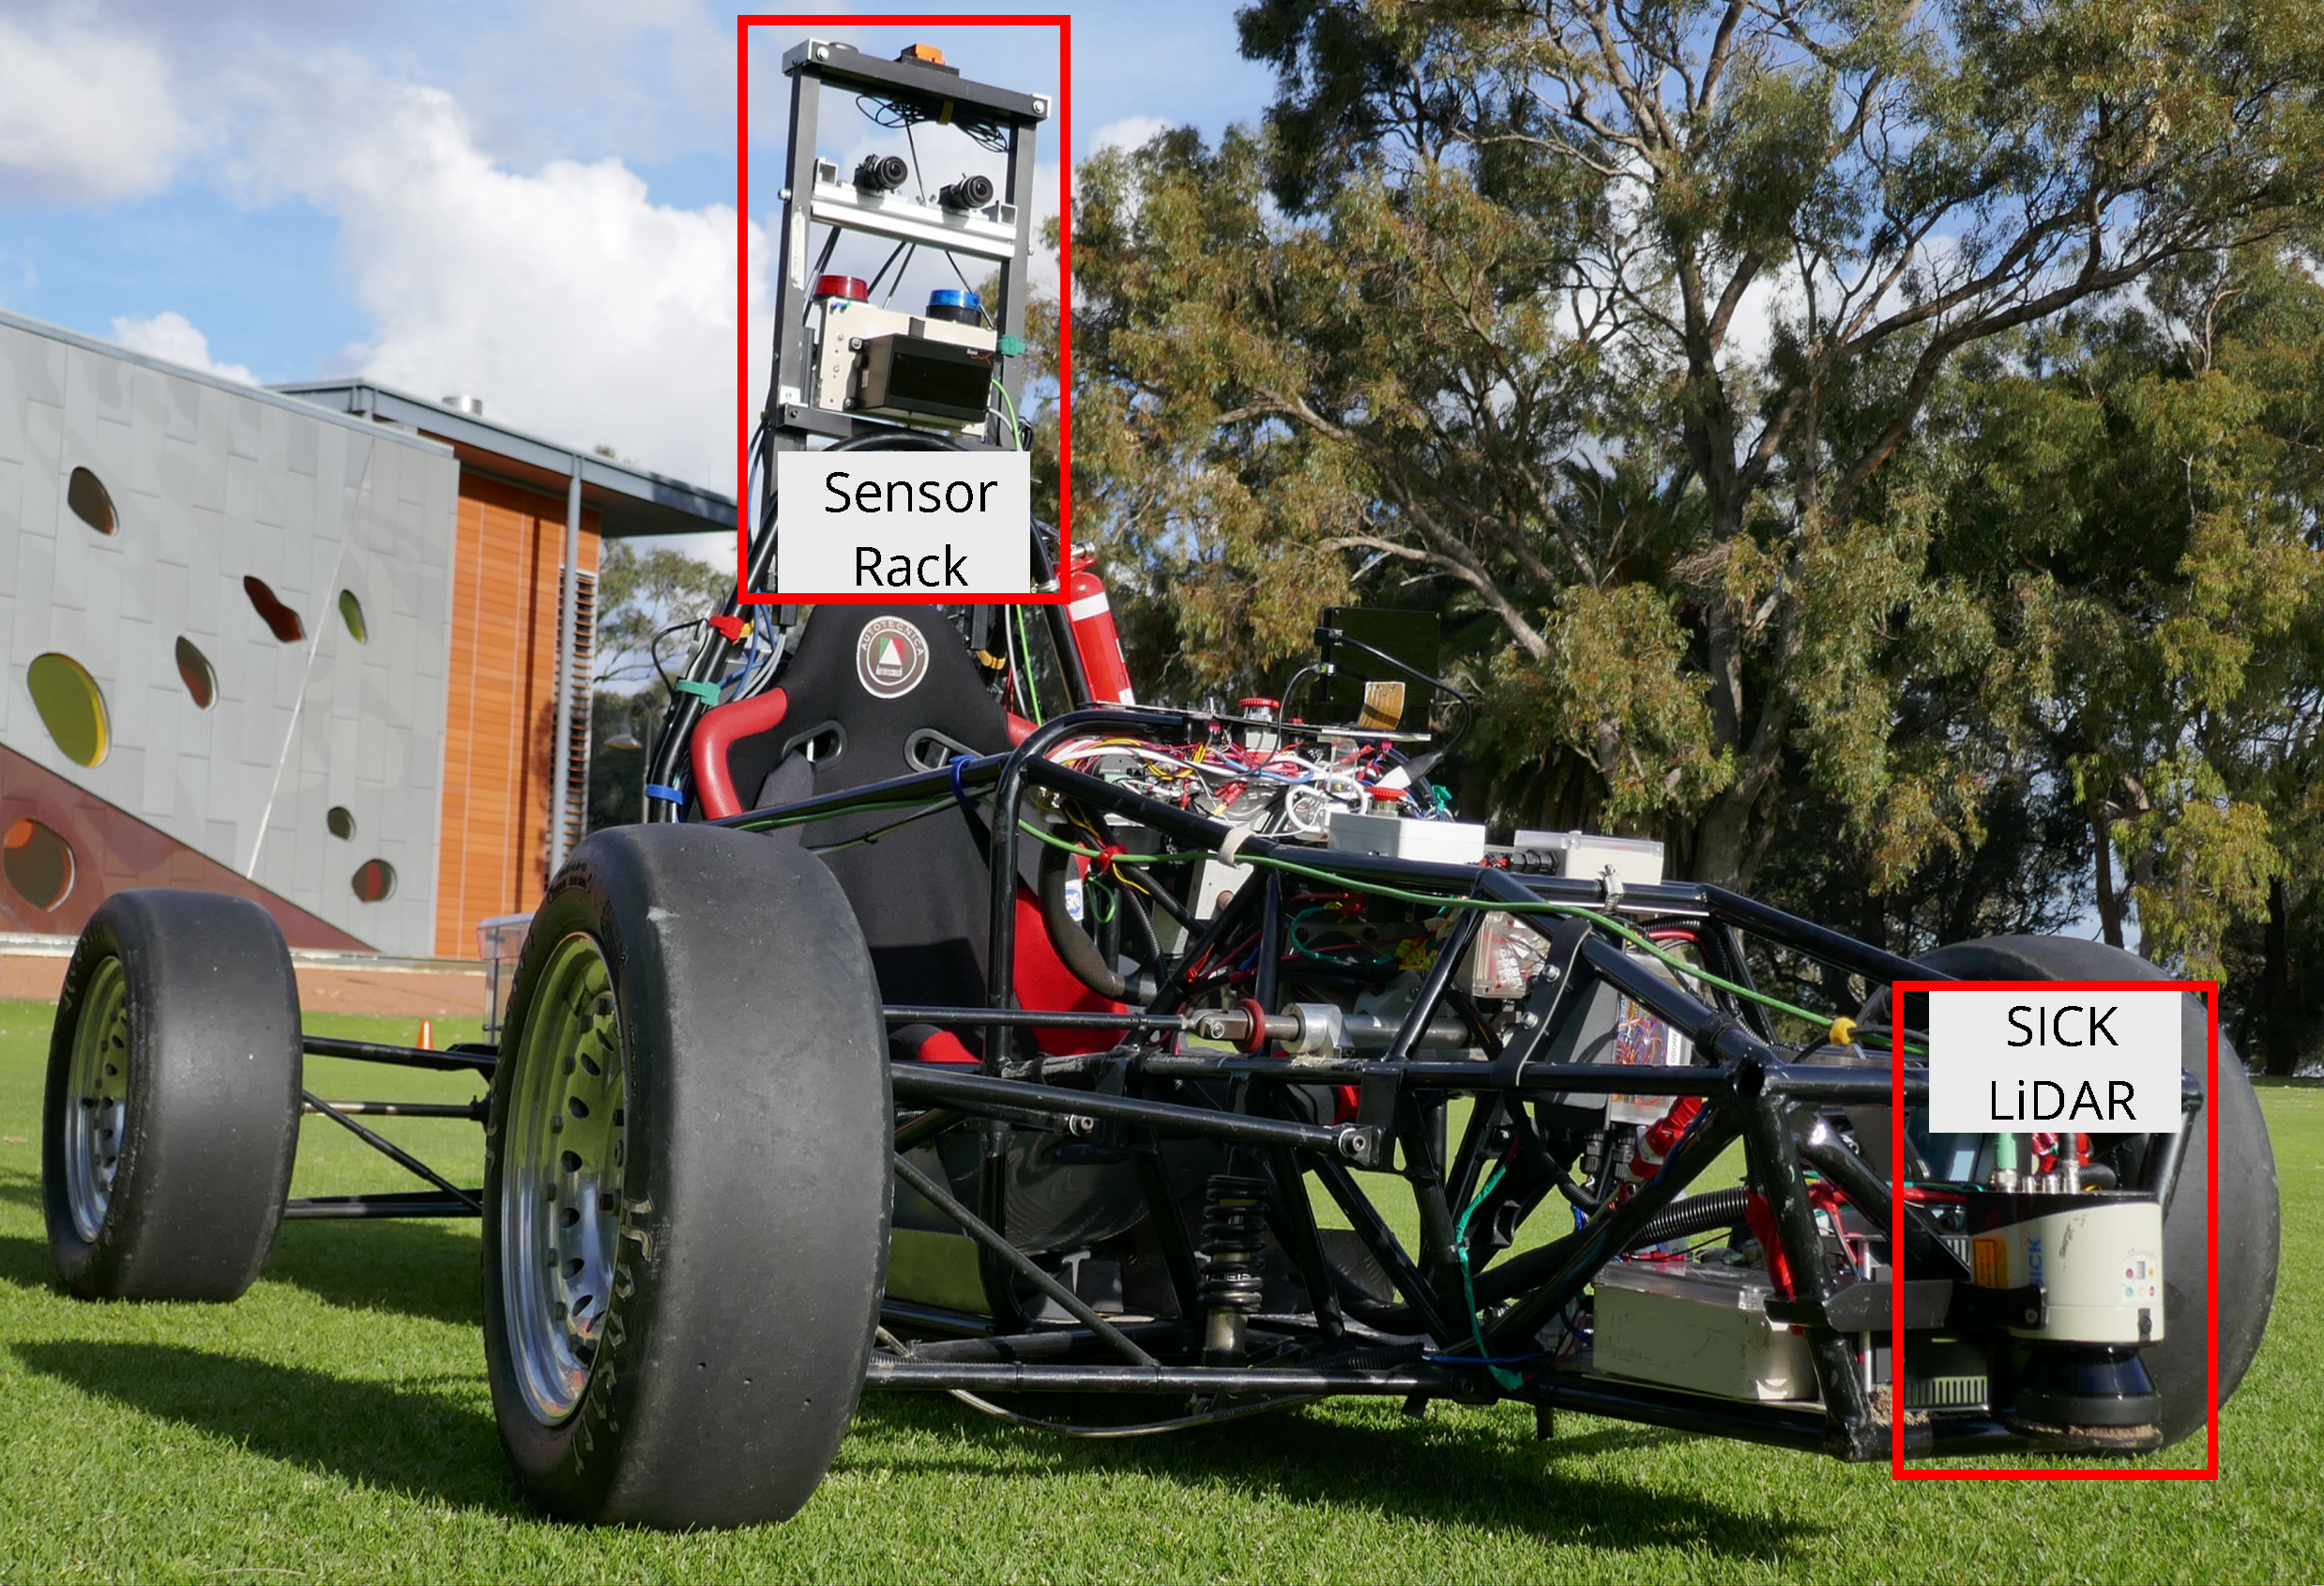
\includegraphics[width=0.7\linewidth]{car}
	\caption{Autonomous SAE Vehicle.}
	\label{fig:7:car}
\end{figure}

For the driverless FSAE project, our goal was to be able to autonomously drive a vehicle around a race track. Initially, this was achieved by placing waypoints along the ideal driving line, as well as ``fence points" to lock out non-driving areas. Maps can either be recorded by human or remote-controlled driving or specified through a Google Maps driven web interface. During autonomous driving, a laser scanner and camera are used for detection of road edges as well as any obstacles on the track. Our current work involves increasing the level of automation to drive a semi-structured (traffic cone or road edge delineated) race track by first automatically driving and mapping the path without prior knowledge of the track and then redriving it, optimised, at greater speed with the assistance of inertial navigation.

Safety systems are essential for a driverless system, as the car weighs more than 250 kg and is capable of driving at a speed of 80 km/h. Both the low-level drive-by-wire, as well as high-level navigation system have independent safety systems built in. These include active geofencing, remote intervention, remote heartbeat and remote emergency stopping, which are implemented through a fail-safe wireless link to a base station as well as through hard-wired buttons on the vehicle itself. 

The previous revision of our framework~\cite{drage_development_2013, lim_modular_2018} had a heavy reliance on a central control module, which required all the sensors and their submodules to function. These submodules were developed over time using different programming languages and are partially redundant, which made integration difficult. First, this was streamlined in an approach whereby each module is programmed with a C++ interface that communicates with either a path planner or a drive control system. Here, we present the integration of this approach with the Robot Operating System~\cite{open_source_robotics_foundation_ros/introduction_nodate} which allows the further separation of functions into ROS nodes and provides a consistent application programming interface (API) for implementation of additional sensors and higher level automation, whilst the original program, now running as a ROS node, deals with critical interfacing and safety functions.

\nomenclature[z-api]{API}{Application programming interface}

Additionally, this approach presents a long-term advantage whereby our framework is made fully open and contributable by students and enthusiasts looking to implement our framework onto their custom-built vehicles. When compared against other autonomous driving frameworks such as Apollo~\cite{baidu_apollo_nodate} and Autoware~\cite{autoware_autoware_nodate} that mostly target commercial vehicles requiring expensive hardware, our approach leverages hardware and fabrication methods that are more affordable. The framework has been integrated with a simulator which provides the ability to test software modifications and algorithms prior to deployment to the vehicle.

Our contributions in this paper are demonstrated through the proposal of our high-level autonomous control system that interfaces through standard, off-the-shelf sensors and equipment. This system is made holistic through the integration of the following features --- real-time localisation through odometry and dead-reckoning; object segmentation and detection using LiDAR and camera; real-time path planning via waypoints or object positioning; visual navigation with odometry, object recognition and tracking, and semantic segmentation; and a hardware-in-the-loop simulator for prototyping verification.  

The remainder of this paper is organised as follows. Section~\ref{sec:7:overview} introduces the system framework with an overview. Section~\ref{sec:7:sensors} describes the sensors that are used. Section~\ref{sec:7:path} presents the path planning approaches used in the system. Section~\ref{sec:7:vision} explains how visual navigation is performed on the system. Section~\ref{sec:7:sim} highlights our driving simulator. Section~\ref{sec:7:bench} describe our system validations, before the concluding remarks are drawn in Section~\ref{sec:7:conclusion}.

\section{System Overview}\label{sec:7:overview}
In order to satisfy the requirements of resiliency, flexibility, extensibility and simple integrations, a publish/subscribe software architecture was used. This allowed for highly decoupled software to be developed, with each component or series of components needing only to conform to the expected message type on the input and output topics.  The use of a publish/subscribe architecture allows for nodes to be easily swapped in and out in order to test different solutions, as well as allowing multiple components to make use of the same data sources without modifying the source, providing simple methods of logging, data capture and data replay.

It was decided to use ROS as the publish/subscribe layer of the application. This decision was influenced heavily by the usage of ROS in the Apollo Auto~\cite{baidu_apollo_nodate} project, as it is shown to be reliable and performant. This also provides a path for upgrades, with a version of ROS modified for automotive use through the addition of shared memory transport for message passing, support for the Protobuf~\cite{google_developers_protocol_nodate} message passing protocol, and the decentralisation of ROS to reduce single points of failure available on an open-source licence. This also allows for any components developed to be more easily ported to the complete Apollo Auto platform at a later stage. In addition, the popularity of ROS ensures that there are a large number of existing modules available for use, allowing the team to focus on the goals stated above, instead of on creating supporting code and utilities.
Based on the desired functionality, it was determined that the publish/subscribe architecture would initially require the nodes and topics outline in Fig.~\ref{fig:7:architecture}.

\begin{figure}[H]
	\centering
	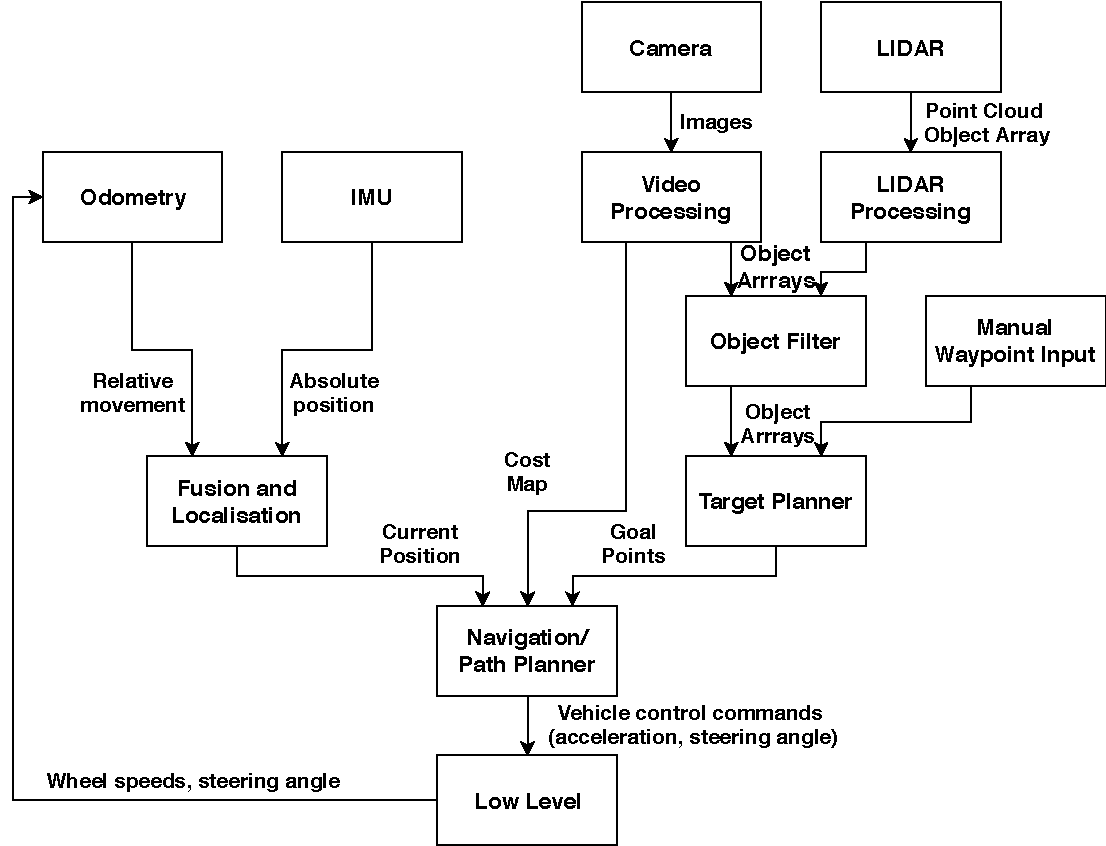
\includegraphics[width=0.8\linewidth]{rosnodes}
	\caption{SAE vehicle software framework.}
	\label{fig:7:architecture}
\end{figure}

We migrated the existing code base of the high-level software system to use the ROS framework in 2018 to reduce the development complexity of the software system. ROS provides low-level device control, implementation of commonly used tools, message passing between processes, and package management~\cite{open_source_robotics_foundation_ros/introduction_nodate}. Instead of creating an independent system where a \textit{broker} would manage the intercommunications between \textit{modules} (programs that have a specific function) ROS readily provides these services. Hence, the user only has to create \textit{nodes} (programs that perform a certain function) that listen and talk to other nodes. Using ROS therefore simplifies the integration process for each individual module in the system. By defining the topic information for messages to communicate, the individual nodes can work together without too much effort in integration. 

More specifically, existing modules in our system presented in~\cite{lim_modular_2018}, including modules for logging, web server and serial communication were replaced with their equivalent ROS packages, as they are often more stable and better supported. All existing messages from the system are converted into ROS messages. The testing for the individual modules therefore only requires minimal changes to the core software.

The ROS version used on the SAE vehicle is currently ROS Kinetic Kame running on Ubuntu 16.04 LTS which will be long-term supported until April 2021.

\section{Navigation Sensors}\label{sec:7:sensors}

\begin{figure}[H]
	\centering
	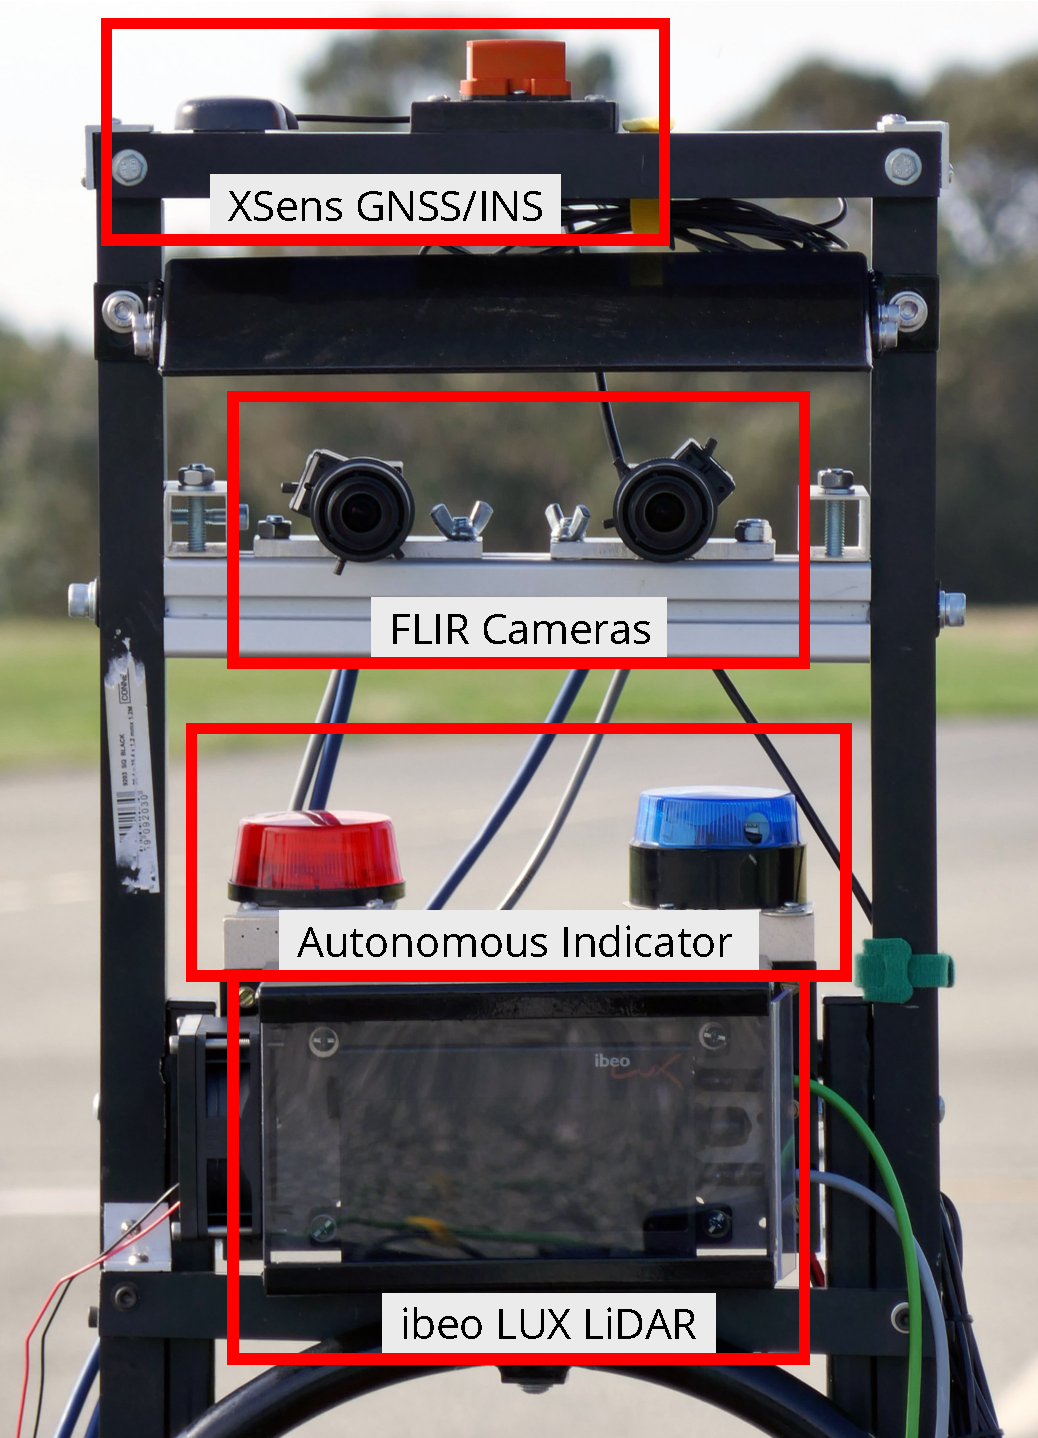
\includegraphics[width=0.45\linewidth]{sensorrack}
	\caption{The SAE vehicle's rack-mounted sensors.}
	\label{fig:7:rack}
\end{figure}

The SAE vehicle performs autonomous driving through a combination of navigation sensors including LiDARs, cameras, wheel odometry and inertial measurement unit (IMU) (as shown in Fig.~\ref{fig:7:car}, with the sensor rack detailed in Fig.~\ref{fig:7:rack}) which are categorised into four categories --- odometry, dead reckoning, LiDAR and camera systems, which are elaborated upon in their individual Sections~\ref{sec:7:odometry} to~\ref{sec:7:camera}.

\subsection{Odometry}\label{sec:7:odometry}
The SAE vehicle has been fitted with Hall Effect sensors on each wheel which send data through a comparator and an \texttt{OR} gate, and generate a pulse train to an Arduino Nano~\cite{arduino_arduino_nodate-1}. The sensors count pulses for each wheel and report them to the low-level controller with timestamps. The linear velocity and rotational velocity are then evaluated by a low-level controller with the feedback from the steering sensor. The accumulated pose information is then combined with the wheel odometry of the SAE car. The goal for implementing this wheel odometry is to provide basic offline localisation within a low-level system and to be further fused with other sensors such as IMU, LiDAR and cameras for a more accurate global positioning.

\subsection{Dead Reckoning}\label{sec:7:dr}
Having an accurate state estimation is crucial for making optimal decisions for future control inputs to effectively navigate the environment. Dead reckoning on the vehicle is achieved through the Xsens MTi-G-710~\cite{xsens_mti-g-710_nodate}, which is an inertial measurement unit (IMU) that is equipped with a global navigation satellite system (GNSS) running at 50 Hz. However, these sensors are susceptible to noise and imperfections which introduce uncertainty to the measurements. Hence, we introduce an extended Kalman filter (EKF) to fuse data from these sensors with that from odometry using a model of the car's dynamics to obtain a more precise estimate of its state. Since the computation of the car's movements requires direction, trigonometric functions are needed. The EKF linearises these non-linear functions using a first-order Taylor series approximation~\cite{yu_derivation_nodate}, where it is approximated according to~\cite{morrell_extended_1997} in equation (\ref{eqn:f_uk}). 
\begin{align}\label{eqn:f_uk}
f(u_k,x_{k-1}) \approx f(u_k, x_{k-1}) + \frac{df(u_k, \mu_{k-1})}{dx_{k-1}}(x_{k-1} - \mu_{k-1})
\end{align}
where $u$ and $\mu$ are the mean and the estimate of $x$, respectively. With an EKF, we calculate the fused covariance values $P_k$ by predicting next state and the next error covariance using the current state and current estimate error covariance. $x_k$ is the current pose at time instance $k$ and $f$ is a non-linear transition function that converts the past state to the current state; state $x$ is composed of the car's $x$-$y$ coordinates and orientation $\varphi$. We perform this as a three-step process, following the descriptions in Section III of~\cite{moore_generalized_2016}:
\begin{enumerate}
	\item Compute the Kalman gain $K$
	\item Perform the correction to find the current state $x_k$, and
	\item Calculate the new process error $P_k$
\end{enumerate}
This is used as the foundation for our experiments on sensor fusion, as described in Section~\ref{sec:7:sensorfusion}.

\nomenclature[g-u]{$\mu$}{Estimate of $x$ [Chapter~\ref{ch:evo}]}
\nomenclature[a-u]{$u$}{Mean} 
\nomenclature[a-k]{$K$}{Kalman gain} 
\nomenclature[g-phi]{$\varphi$}{Vehicular orientation} 

\subsection{LiDAR System}
The vehicle utilises an array of Light Distance and Ranging (LiDAR) systems. This consists of a SICK LMS111-1010~\cite{sick_ag_lms111-10100_nodate} and an ibeo LUX 4~\cite{autonomoustuff_ibeo_nodate} connected through an Ethernet switch to the Nvidia Jetson TX1. The LMS111 scans a single layer at 50 Hz while the LUX scans four layers at 10 Hz featuring in-built object detection and tracking. 
The data is published by each of the LiDAR's ROS drivers and processed to achieve desired functionalities.

The LMS111 is mounted forward-facing on the front of the vehicle at 15 cm above the ground to obtain a \ang{270} field of view, suitable for detecting close obstacles and scans a plane close to horizontal. The point cloud is sorted and then from left to right; each point is assigned a cluster identification number based on distance to the next point and the angle between it and the next point relative to the laser. This delivers accurate obstacle detection with features such as cluster size indicating the size of the obstacle, allowing for classification of obstacles (such as a cone). The LUX is mounted above the driver and pitched towards the ground slightly such that the lower layer scans the ground 20 metres ahead of the vehicle. It is utilised to achieve road edge and object detection at a distance. 

Road edge detection is achieved by analysing the depth information in one of the layers and checking it for both smoothness and slope. The central data points and those near them are considered and checked to confirm that they meet the slope criteria (the road should be relatively flat so no great changes in depth should be noted in a line). Iteratively, further and further points are considered in a stepwise process where the correlation coefficient is considered at each point. The road edge is the point at which the correlation coefficient is the highest whilst the slope condition is still being met. This approach was improved with the implementation of a Kalman filter which creates a time-averaged estimate of the road edge-position assisting in the prediction of the current road edge. A detailed description of our methods is presented in~\cite{drage_lidar_2015}.

\begin{figure}[H]
	\centering
	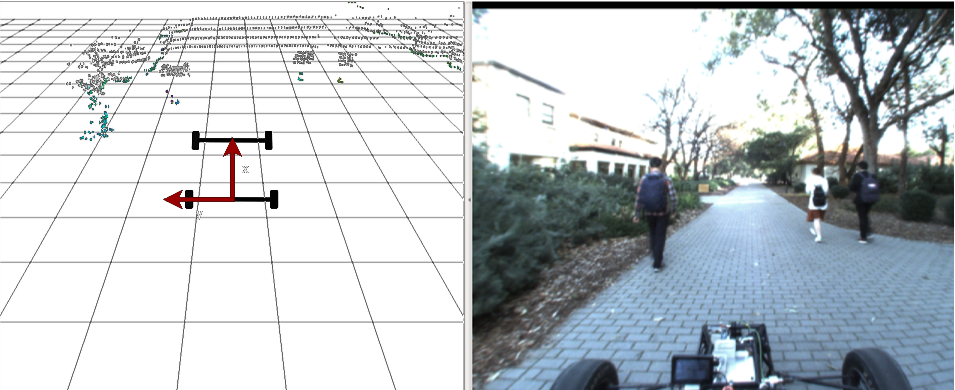
\includegraphics[width=0.8\linewidth]{pointcloud}
	\caption[Captured scene with its instantaneous LiDAR point cloud]{Point cloud generated from the LMS111 (coloured) and the LUX (4-layers, white) (left) and the scene where it was captured (right).}
	\label{fig:7:pointcloud}
\end{figure}

The in-built object detection and tracking of the LUX will be used for fusion with the obstacles reported through processing of the LMS111's data. The comparison of positions of objects reported by the LUX and LMS111 will increase the likelihood of detecting an object. The LMS111 giving information on the objects on a low and horizontal plane and the LUX giving information of objects in the mid to far range. In turn, this object information will also be fused with that of the camera vision. 
We use both LiDARs to collectively generate a point cloud as illustrated in Fig.~\ref{fig:7:pointcloud}, captured during a test run. 
The LMS111 point cloud is coloured based on its intensity, retrieving information on the reflectivity of the surface struck by each point. The LUX is scanning layers onto the path in the distance while also picking up a large amount of detail from the surrounding vegetation as pedestrians walk past.

\subsection{Camera System}\label{sec:7:camera}
A pair of FLIR Blackfly GigE~\cite{flir_blackfly_nodate} cameras are mounted on the vehicle's frame to perform tasks related to visual navigation, such as semantic segmentation and visual odometry. These cameras are fitted with Fujinon f/1.2, 2.8--8 mm wide-aperture varifocal lenses~\cite{flir_fujinon_nodate}, and are individually capable of capturing a wide field of view. To suit our application, these cameras use 1.3 megapixel 1/3" global shutter CCD image sensors that will not be affected by any distortions caused by the rolling shutter effect~\cite{liang_analysis_2008}. The cameras are connected to a Gigabit Ethernet switch that connects to the Jetson TX1, interfacing them through Blackfly's ROS node where it is configured to record at 10 Hz per channel.

\nomenclature[z-ccd]{CCD}{Charge-coupled device}

At the time of writing, the use of stereoscopic vision for autonomous driving is still subject to evaluation. Our application focuses on using monocular vision that is paired with measurements from the LiDAR system in order to achieve depth perceptions. The methods that we use for semantic segmentation and visual odometry for this paper currently do not require a stereoscopic setup. Our implementation of these methods is further described in Section~\ref{sec:7:vision}.

\section{Path Planning}\label{sec:7:path}
We have programmed the control system to deliver path planning routines to drive either through a series of predefined waypoints, or in between a series of traffic cones placed on either side of the vehicle.

\subsection{Waypoint Driving}\label{sec:7:waypoint}
The underlying idea behind waypoint driving is to drive a set of predefined points in between the starting position $P_1$ ($x$ = 0, $y$ = 0 and orientation $\varphi$ = 0) to the destination position $P_2$, which can be obtained through the differences in GPS coordinates. These waypoints can either be stored in Cartesian coordinates in an array or in our test case, they are selected based on the driver's preference by selecting position points on RViz~\cite{kam_rviz:_2015}, which are then confirmed on the console. To ensure that all points can be driven smoothly with the consideration of the correct heading to the subsequent point, a spline approach has been implemented within this design to generate the desired path.

Once the waypoints are chosen, two static paths are shown on RViz (see Fig.~\ref{fig:7:waypoint}). The first path (green) consist of straight lines that interlink all the points with the arrow at the end showing the destination heading. The second path (purple) is the desired path which consists of a smoothed curvature that passes through all of the waypoints, the generation of this path is based on the Hermite spline interpolation technique~\cite{de_boor_practical_1978} with the required parameters which are the four vectors:
\begin{enumerate}
    \item Current position, $P_1$
    \item Target position, $P_2$
    \item Tangent of departure from current position, $T_1$
    \item Tangent of approach from target position, $T_2$
\end{enumerate}
Along with four Hermite basis functions $H_n(u)$
\begin{subequations}
	\label{eqn:hermitebasis}
	\begin{align}
	H_1(u) &= 2u^3-3u^2+1 \\
	H_2(u) &= -2u^3+3u^2 \\
	H_3(u) &= u^3-2u^2+u \\
	H_4(u) &= u^3-u^2
	\end{align}
\end{subequations}
where $0 \leq u \leq 1$ which represents the start to finish motion. We then construct the resultant path $f$ by calculating the product between the vectors and the Hermite basis functions
\begin{align}\label{eqn:hermite}
f(x,y,\varphi) = H_1P_1 + H_2P_2 + H_3P_3 + H_4P_4
\end{align}

\nomenclature[a-H]{$H_n$}{Hermite basis function} 
\nomenclature[a-P]{$P_x$}{Position at $x$} 

\begin{figure}[H]
	\centering
	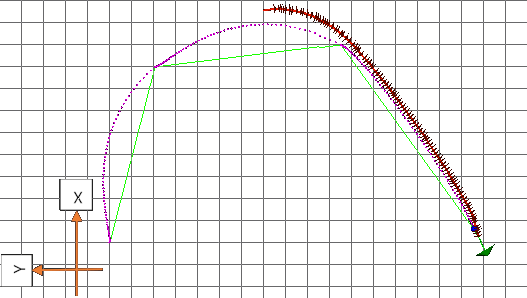
\includegraphics[width=0.6\linewidth]{waypoint}
	\caption{Calculated waypoints on RViz with inputs from~\eqref{eqn:hermitebasis} and~\eqref{eqn:hermite}.}
	\label{fig:7:waypoint}
\end{figure}

The actual simulated driving pattern (red line) is determined based on the distance measurement between the current position of the vehicle against the desired path (purple) with a predefined tolerance range, and limited maximum turning angle ranged between $\pm\ang{25}$. The desired path is constituted by a finite number of points generated from the Hermite spline interpolation. To avoid oversteering or understeering, we compute the slope differences for both the driving path and the desired path.  With this logic in place, the vehicle is either turning left ($\varphi$ \textgreater\ \ang{0}), right ($\varphi$ \textless\ \ang{0}) or moving straight either at a constant speed or slowed speed for a sharper turn in order to reach the goal point ($\varphi$ =\ \ang{0}).

\subsection{Cone Driving}\label{sec:7:cone}
The current iteration of the path planning procedure uses obstacle detection of the cones to determine the correct path. This algorithm is similar to our solution in~\cite{lim_modular_2018}, but simplified to allow for quicker calculation. Our cone driving module accepts cone locations from either the map, LiDAR or camera, classifying them as objects. Then, the vehicle navigates to drive within the track formed by cones safely without collision. Using a range of the maximum turning circle of the car, of both a left-hand turn and right-hand turn, it then looks at which predicted paths will intercept cones. The vehicle dynamics are thus limited during motion planning such that the steering angle does not exceed \ang{25}. Our algorithm will iterate through all cones within the car's range and calculate the best collision-free path to undertake, as detailed in Algorithm~\ref{algo:7:cones}.

\begin{algorithm}
	\begin{flushleft}
		\caption{Cone driving}\label{algo:7:cones}
		\begin{algorithmic}[1]
			\Procedure{ConeDrive}{cones in range}
			\State init \textit{steering\_range} to [-25,25]
			\For{all \textit{cones} in \textit{range}}
			\State evaluate \textit{collision\_range} with \textit{cone}
			\State exclude the \textit{collision\_range} from \textit{steering\_range}
			\EndFor
			\If{\textit{steering\_range} is empty}
			\State stop
			\ElsIf{all \textit{steering\_range} $\leq$ \textit{threshold}}
			\State select largest \textit{steering\_range}
			\ElsIf{all \textit{steering\_range} $>$ \textit{threshold}}
			\State select \textit{steering\_angle} with minimum change in current direction
			\EndIf
			\State drive toward centre of \textit{steering\_range}
			\EndProcedure
		\end{algorithmic}
	\end{flushleft}
\end{algorithm}

\section{Visual Navigation}\label{sec:7:vision}
The vehicle is capable of performing visual navigation tasks through a combination of semantic segmentation, visual odometry and visual cone detection that is decided depending on the application requirements. These tasks commonly rely on the OpenCV~\cite{opencv_opencv_2016} library, utilising functions such as handcrafted feature detection, general image processing and transforming. It achieves a visual perception of the driving environment through the camera system as described in Section~\ref{sec:7:camera}.

\subsection{Road and Lane Detection}\label{semseg}
Our system uses either semantic segmentation or edge detection to detect road edges and lane markings, depending on the environment's complexity. Using semantic segmentation also enables obstacle recognition which can be integrated with the LiDAR system. Environments are complex when there is a lack of uniformity in pose, features and illumination. While it is possible to solely rely on modules within OpenCV here, the performance of using handcrafted features alone for image recognition is restricted by variations in image quality, brightness, and contrast. In order to improve its performance under these environments, we selected SegNet~\cite{badrinarayanan_segnet:_2017} for semantic segmentation due to its high compatibility and ease of implementation. Its ability to perform pixel-wise classification for road scene objects complements the drawbacks of a single image processing scheme.

The architecture of SegNet uses a convolution encoder and decoder setup that classifies objects into one of the following classes --- sky, building, column-pole, road-marking, road, pavement, tree, sign-symbol, fence, vehicle, pedestrian and bicyclist; with a class average classification accuracy of 65.9\%~\cite{badrinarayanan_segnet:_2017}. Our application uses SegNet whereby road, road markings, and pavement are classified (see Fig.~\ref{fig:7:segnet}), which is useful for road edges detection. However, OpenCV is simultaneously used to perform image processing, with the first step being camera calibration to get an undistorted image. This is achieved using a chessboard image and finding its corners to get two accumulated list --- a 3D point in real-world space and a 2D point in an image plane. We then use the camera calibration function in the OpenCV library to obtain the camera calibration and distortion coefficients. Our experiments using SegNet for autonomous driving was performed in~\cite{k._l._lim_implementation_2017}, where we have evaluated its segmentation accuracy in our test environment through the calculation of its pixel accuracy (PA).
\begin{align}\label{eqn:PA}
\textrm{PA} = \frac{\sum_{i}n_{ii}}{\sum_{i}t_i}
\end{align}
where $n_{ii}$ represents the number of classified class $i$ pixels correctly classified to belong in class $i$, and $t_i$ represents the total number of pixels in class $i$ belonging in the ground truth.

\nomenclature[s-i]{$i$}{Classified class (semantic segmentation)}   

\begin{figure}[H]
	\centering
	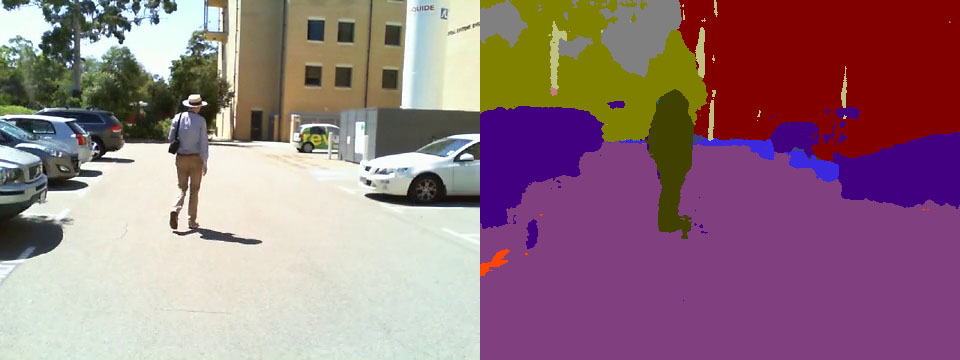
\includegraphics[width=0.8\linewidth]{segnet}
	\caption[Semantic segmentation results from test drive]{Semantic segmentation results during a test drive. This scene resulted in a pixel accuracy of 99.31\%.}
	\label{fig:7:segnet}
\end{figure}

The road edges detection process finds lane markings at both sides of the car. We have noted that lane marking detection can also be performed solely using OpenCV functions, especially in non-complex, uniform environments with minimal illumination variations, thereby reducing its computation requirements. Algorithm~\ref{algo:7:lanes} describes our approach.

\begin{algorithm}
	\begin{flushleft}
		\caption{Road and Lane Detection}\label{algo:7:lanes}
		\begin{algorithmic}[1]
			\Procedure{LaneDetect}{\textit{histogram\_vector} from camera}
			\State undistort \textit{image\_frame} from lens distortions
			\State Sobel filter \textit{image\_frame} as \textit{filtered\_image}
			\State threshold \textit{filtered\_image} as \textit{binary\_image}
			\State obtain \textit{histogram\_vector} for \textit{binary\_image} on $y$-axis
			\State split \textit{histogram\_vector} into left\_half and right\_half
			\For{each \textit{histogram\_vector}}
			\State find \textit{peak\_position} on $y$-axis
			\State init \textit{sliding\_window} at bottom of image at \textit{peak\_position}
			\While{\textit{sliding\_window} not at \textit{top\_of\_image}}
			\State find \textit{mass\_center} of \textit{sliding\_window} as \textit{line\_point}
			\State move \textit{window} to the \textit{mass\_center}
			\State move \textit{window} iteratively on $x$-axis towards \textit{top\_of\_image}
			\EndWhile
			\State fit \textit{line\_point} with second-order polynomial
			\EndFor
			\EndProcedure
		\end{algorithmic}
	\end{flushleft}
\end{algorithm}

The lane distances are obtained using pixel values that are converted into metres, and its scaling factors are according to Australian road width standard of 3.3 to 3.5 metres. However, this image processing approach might fail when the lane markings are not clear or there are no lane markings. Therefore, using SegNet's results can effectively mitigate this drawback due to its ability to robustly detect and classify road and lane markings, whereby the same road distance calculation can be applied to find the vehicle's distance to the road edges.

\subsection{Visual Odometry}\label{sec:7:vo}
Our system implements ORB-SLAM2~\cite{mur-artal_orb-slam2:_2017} as our baseline algorithm for visual odometry based on its use of Oriented FAST and rotated BRIEF (ORB) features for mapping, tracking and place recognition. ORB features are similar to Binary Robust Independent Elementary Features (BRIEF) with an extra feature of introducing rotation invariance and noise resistance, while utilising Features from accelerated segment test (FAST) for corner detection. This results in a balanced compromise between accuracy and computation footprint, making it desirable for our hardware setup. Although initially proposed as a visual simultaneous localisation and mapping (SLAM) algorithm, our ORB-SLAM2 application focuses on visual odometry as we do not implement its loop closing feature. To further increase the efficiency of this algorithm for our specific needs, a new set of vocabularies were trained using the images collected from the cameras mounted on the car. This reduces the size of vocabularies, which results in improved memory footprint. The Jetson TX1's 256-core embedded GPU is being used to improve image processing through parallelisation. The original ORB-SLAM2 was not adapted for this acceleration. In order to boost runtime performance, the applied ORB-SLAM2 has been rewritten to adapt CUDA~\cite{nvidia_corporation_parallel_2016} and thus utilise the GPU on the TX1~\cite{chen_yunchih/orb-slam2-gpu2016-final_2019}. Fig.~\ref{fig:7:vo} illustrates an experiment with ORB-SLAM2 on a path segment as shown in (a), with its generated path in (b) through the tracking of features along subsequent frames.

\begin{figure}[H]
	\centering
	\begin{subfigure}[b]{0.45\textwidth}
		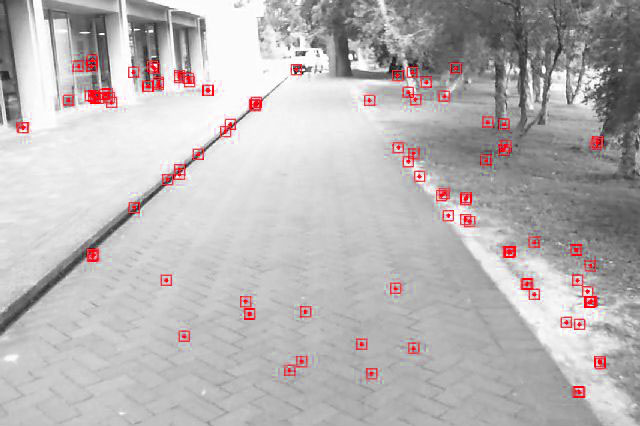
\includegraphics[width=\textwidth]{vo}
		\caption{Tracked keyframes}
		\label{fig:7:vo:1}   
	\end{subfigure} 
	\hspace{1em}         
	\begin{subfigure}[b]{0.45\textwidth}
		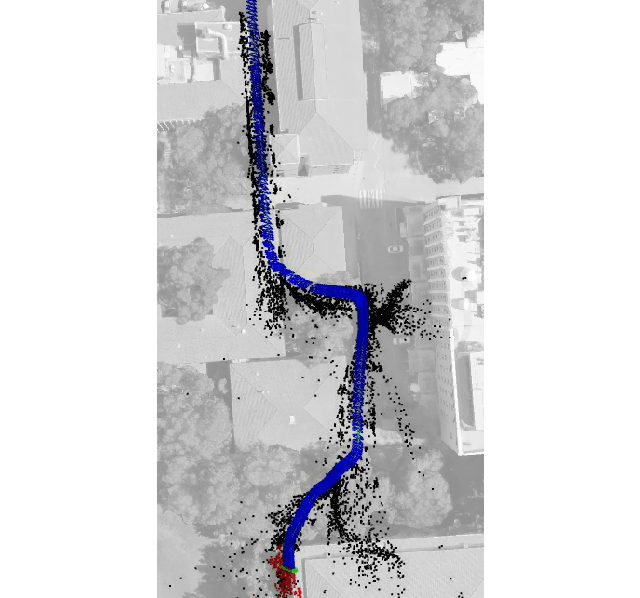
\includegraphics[width=\textwidth]{os_overlay}
		\caption{Resultant path}
		\label{fig:7:vo:2}
	\end{subfigure}             
	\caption[ORB-SLAM2 experiment]{ORB-SLAM2 experiment showing (a) tracked keyframes as red points that results in (b) the generated path in blue with the said tracked features as red dots, overlaid on satellite imagery.}
	\label{fig:7:vo}
\end{figure}

\subsection{Cone Detection}\label{sec:7:conedetect}
Handcrafted features that combine a linear classifier are utilised for cone detection using OpenCV. We use the histogram of oriented gradients (HOG) descriptor across an image to find and segregate regions of interest (ROIs) that may encompass a cone, which is then used as inputs for a support vector machine (SVM) classifier. For all regions that are positively classified, the hue layer is thresholded with an orange value, as our system is benchmarked using orange cones. We finally apply a histogram to the thresholded image and then obtain the position of the cone within the image frame. However, in order to fuse this classification result with other sensors, the detected cones must be presented in the global reference frame. This is done by applying a perspective transform to the image, and with the assumption that the vehicle is driving on a flat plane. The position of the cones in the global frame can then be obtained by projecting these cones onto a horizontal ground plane.   

\nomenclature[z-hog]{HOG}{Histogram of oriented gradients}

In order to reduce the effect from variations in brightness caused by the different sunlight angles, more samples must be included in the training process of the SVM. This significantly degrades the runtime performance of the entire system while offering only a minor accuracy improvement. Because of this, we designed a convolutional neural network (CNN) to provide a flexible feature extraction method to adapt this variation in the environment. This network has two convolutional layers and two fully-connected layers, which are used for detecting cones. In order to run the visual cone detection process smoothly along with all other modules in the system, we designed the network to be simple with a small footprint. Using this CNN yielded increased detection accuracies as compared to the SVM approach while offering similar runtime performance~\cite{girshick_region-based_2016}. 

\section{Hardware-in-the-Loop Simulation}\label{sec:7:sim}
Simulation is a cornerstone of autonomous vehicle testing, allowing high-level software such as image processing and path planning to be tested in predefined scenarios on a much faster schedule than is possible with hardware testing. In addition, the use of autonomous driving simulations allows for testing to be performed in faster than real time, and for testing to be scheduled and the results reviewed at a later time. 

We designed a hardware-in-the-loop (HIL) simulation system, whereby an interface between the high-level software of the autonomous SAE vehicle and the CARLA driving simulator~\cite{dosovitskiy_carla:_2017} allows software components such as localisation and path planning to be tested in a simulated environment, resulting in faster iterations as tests can be conducted at any time that is convenient. This interface consists of a ROS node that retrieves environment data such as a camera feed and LiDAR point cloud from CARLA and sends movement commands to CARLA. Due to the message passing system used by ROS, this interface can easily generate and consume the outputs and inputs expected by other ROS nodes without requiring changes to the application, even across multiple devices, and allows for the application architecture in Fig.~\ref{fig:7:simarchitecture}. This allows CARLA to be run on a more powerful computer more suited to generating a simulated environment while still allowing for the Jetson TX1 to be used to run the SAE vehicle software in order to maintain as realistic an environment and workload as possible, as the control hardware and software on the simulator is identical to the ones used in the real vehicle. In addition, the simulation node handles input from a Logitech G920 racing wheel~\cite{logitech_logitech_2019} and simulates the low-level safety systems in order to allow overriding autonomous functions using manual inputs in a similar manner to what is possible on the SAE vehicle.

\begin{figure}[H]
	\centering
	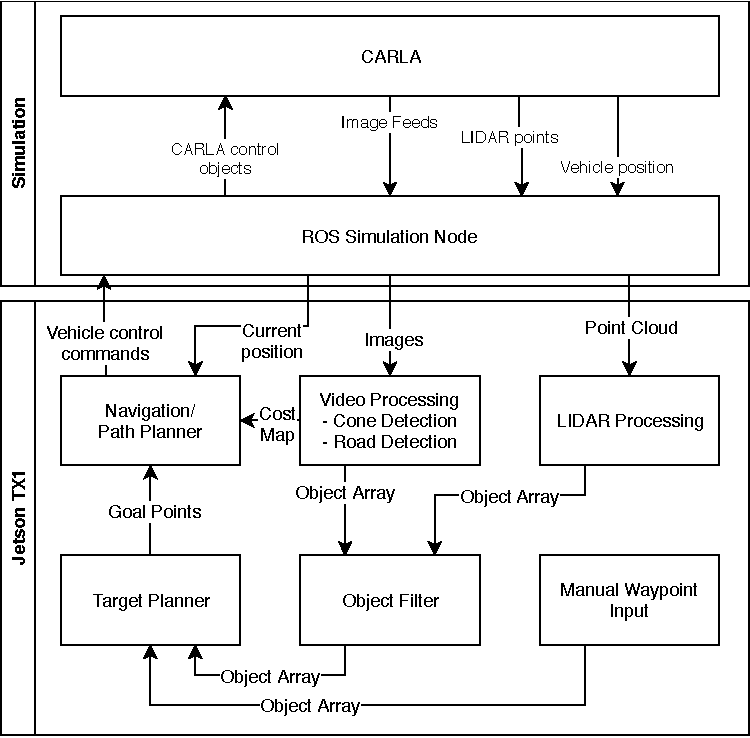
\includegraphics[width=0.7\linewidth]{simarchitecture}
	\caption{Simulation software framework.}
	\label{fig:7:simarchitecture}
\end{figure}

\section{System Validation}\label{sec:7:bench}
In order to verify our system, we conducted experiments relating to sensor fusion for dead reckoning, waypoint and cone driving, and the driving simulator, which are elaborated individually in Sections~\ref{sec:7:sensorfusion} through~\ref{sec:7:benchdrive}.

\subsection{Sensor Fusion}\label{sec:7:sensorfusion}
The odometry measurements are compared to the fused odometry and IMU position estimate using our approach described in Section~\ref{sec:7:dr}. To gather the data, the vehicle was driven in a relatively straight path on an even plane and as a result the $z$ coordinate was omitted. In Table~\ref{tbl:7:odometry}, we hence measured and calculated the displacement of the car's state $\Delta x_k$ and its error covariance $P_k$ across three time instances $k$ measured in seconds. We then compared the values obtained through pure wheel odometry (no IMU fusion) against that from the EKF (with IMU fusion); these values are expressed in Cartesian coordinates ($x$,~$y$) and are measured in metres.

\nomenclature[a-k]{$k$}{Time instance [Chapter~\ref{ch:evo}]}
\nomenclature[a-n]{$\Delta x$}{State displacement}      
\nomenclature[a-P]{$P_k$}{Error covariance at instance $k$ [Chapter~\ref{ch:evo}]}

\begin{table}[H]
	\caption{Displacement \& Error Covariance Comparison}%, With and Without IMU Fusion}
	\label{tbl:7:odometry}
	\centering
	\begin{tabular}{lccc}
		\toprule
		IMU Fusion & $k$ & $\Delta x_k$ & $P_k$\\
		\midrule
		No  & 50.88   & (1.430, 0.030)    & (0.0160, 0.0160)  \\
		& 100.91  & (41.070, 13.934)  & (0.0160, 0.0160)  \\
		& 150.89  & (58.000, 27.680)  & (0.0160, 0.0160)  \\
		\midrule
		Yes     & 50.88   & (1.436, 0.025)    & (0.0130, 0.0134)   \\
		& 100.91  & (41.073, 13.901)  & (0.0132, 0.0132)   \\
		& 150.89  & (57.970, 27.658)  & (0.0132, 0.0133)   \\
		\bottomrule
	\end{tabular}
\end{table}

The results in Table~\ref{tbl:7:odometry} shows an improvement in the certainty of positioning, whereby sensor fusion has performed corrections to the coordinates and improved the covariances in $x$ and $y$. In our tests, the combination is sufficiently accurate for this application.

\subsection{Waypoint Driving}\label{sec:7:benchway}
We carried out our experiments for waypoint driving by measuring its path planning accuracy through the calculation of waypoints across several driving scenarios as shown in Fig.~\ref{fig:7:expwp}. Figure legends are as presented in Section~\ref{sec:7:waypoint}. This accuracy is quantified by the car's projection error $\epsilon_P$ (the maximum deviation of the path projection from the ground truth), and its root-mean-square error $\epsilon_\textrm{rms}$.
\begin{align}
\epsilon_\textrm{rms} = \sqrt{\frac{\sum\limits_{i=1}^{n} (D_i - M_i)^2}{n}}
\end{align}
where $n$ denotes the total number of records; $D_i$ and $M_i$ denotes the distance of the ground truth and the projected path, respectively at record $i$.  

\nomenclature[g-e]{$\epsilon$}{Error}
\nomenclature[a-k]{$M$}{Projected distance}

\begin{figure}[H]
	\centering
	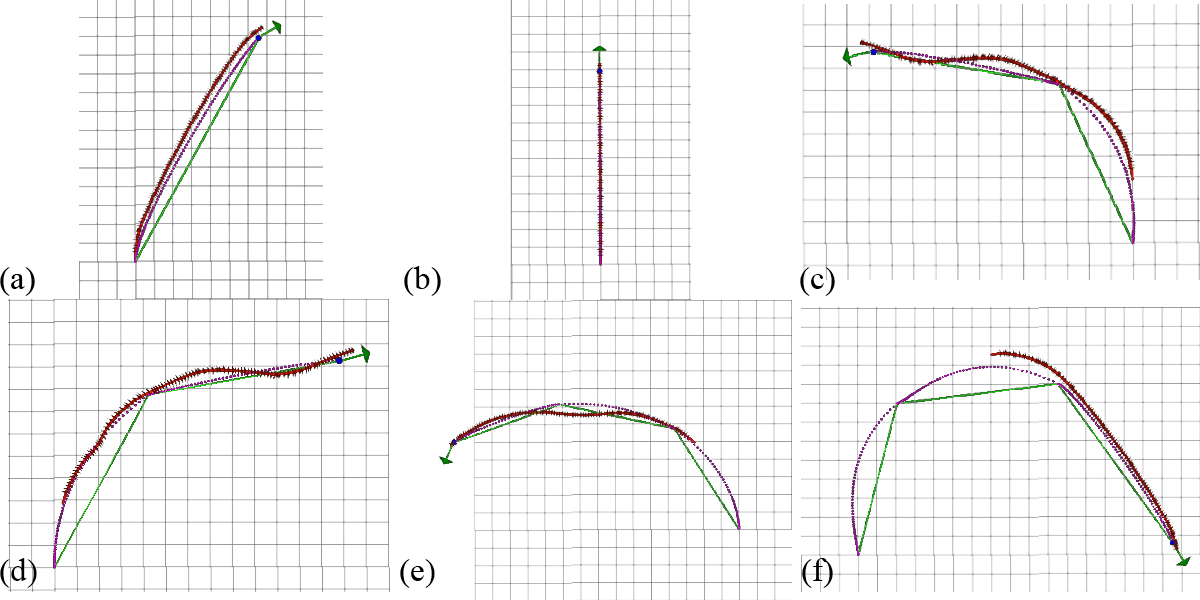
\includegraphics[width=\linewidth]{wp2}
	\caption[Generated path projections, ground truth and linear displacements]{Generated path projections $M_i$ (red), its ground truth $D_i$ (purple) and the linear displacements of waypoints (green). [Grid size: $\SI{1}{\meter}\times\SI{1}{\meter}$]}
	\label{fig:7:expwp}
\end{figure}

Distance error measurements are shown in Table~\ref{tbl:7:waypoint}, while heading angle deviations were found to be insignificant.

\begin{table}[H]
	\caption{Error and Distance Measurements from Fig.~\ref{fig:7:expwp}}
	\label{tbl:7:waypoint}
	\centering
	\begin{tabular}{cccc}
		\toprule
		Fig.~\ref{fig:7:expwp} & $\epsilon_p$ (m) & $M_i$ (m) & $D_i$ (m) \\
		\midrule
		(a)  & 0.316 & 13.895 & 13.579 \\
		(b)  & 0.000 & 10.895 & 10.895 \\
		(c)  & 0.412 & 15.053 & 14.158 \\
		(d)  & 0.368 & 15,263 & 14.482 \\
		(e)  & 0.474 & 13.895 & 14.105 \\
		(f)  & 0.626 & 14.053 & 13.737 \\
		\bottomrule
	\end{tabular}
\end{table}

Using the values of $M_i$ and $D_i$ in Table~\ref{tbl:7:waypoint}, $\epsilon_\textrm{rms}$ was calculated to be 0.525 m, which is 85\% accurate when compared to the average transverse track width of 3.5 m. This accuracy indicates that $D$ is relatively close to $M$ across the total $i$ records. Additionally, the increase in track complexity (such as through the addition of sharper turns and more segments) contributes to a greater increase in $\epsilon_p$, as compared to the increase of $(D_i-M_i)$. As expected, $\epsilon_p$ is non-existent when a perfectly straight path is generated as shown in Fig~\ref{fig:7:expwp}b.

\subsection{Cone Driving}\label{sec:7:benchcone}
Cone driving on the car follows the setup as prescribed by the standards set by Formula Student Germany's Track Marking and Skidpad for Dynamic Events (DE6.3/DE6.4)~\cite{formula_student_germany_gmbh_fsg_2018}. Each cone measures $228 \times 228 \times 325$ ($l\times w \times h$) \si{\milli\meter} and they are placed as pairs 5 \si{\meter} apart, creating a track width of 3.5 \si{\meter}, as illustrated in Fig.~\ref{fig:7:conedrone}.

\begin{figure}[H]
	\centering
	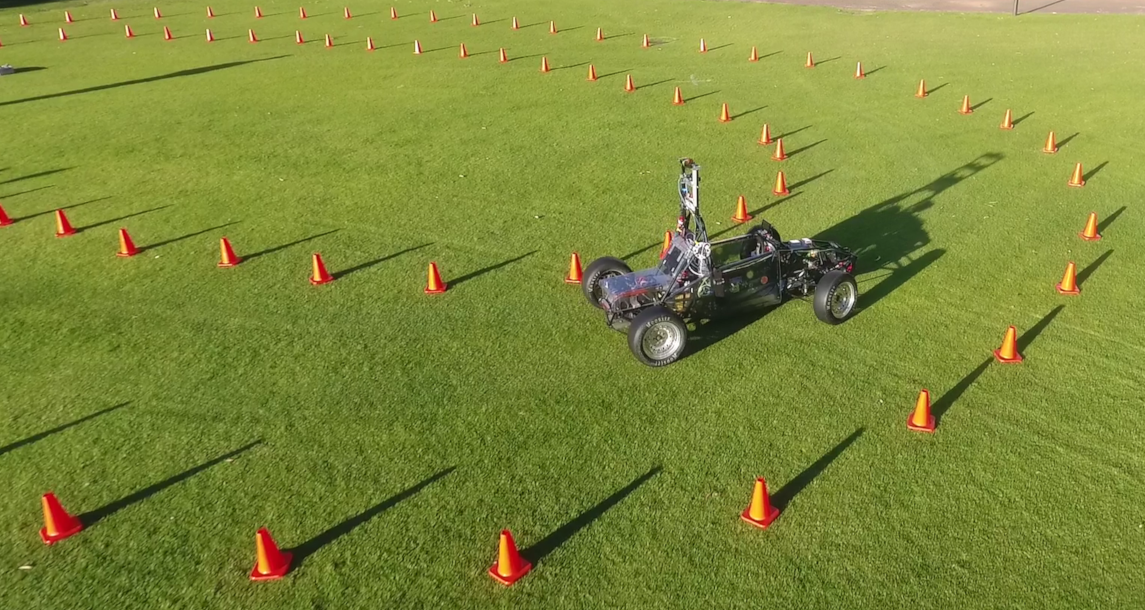
\includegraphics[width=0.8\linewidth]{dronecones_cropped}
	\caption{Experimental setup for cone driving.}
	\label{fig:7:conedrone}
\end{figure}

The system obtains the positions of the cones through the combination of LiDAR and vision processing. Data from the LiDAR is simultaneous to visual cone detection to provide a more robust solution to cone positioning. In our experiments, the speed of the car is limited to 5 \si{\meter\per\second} due to safety considerations.  

\begin{figure}[H]
	\centering
	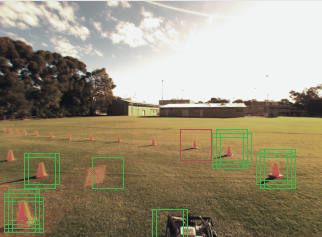
\includegraphics[width=0.7\linewidth]{svm2.png}
	\caption{Visual cone detection showing the detected cones in bounding boxes.}
	\label{fig:7:svm}
\end{figure}

To detect cones in the vicinity, we first apply the process described in Section~\ref{sec:7:conedetect} to find a suitable path to navigate. Fig.~\ref{fig:7:svm} shows the detected cones in bounding boxes, which are red upon detection turns green as it passes the colour filter. The accuracy of visual cone detection for our initial training and test sets are good, at 96.3\% and 92.1\% respectively, with its F\textsubscript{1} score as calculated in Table~\ref{tbl:7:cone}, which are given in their mean, best and worst cases as measured from each frame across different lighting conditions. These results imply that our classifier is highly accurate under certain conditions and with a mean F\textsubscript{1} score of 0.85, our visual cone detection algorithm is therefore deemed suitable for the system. 

\begin{table}[H]
	\caption{F\textsubscript{1} Scores for Visual Cone Detection}
	\label{tbl:7:cone}
	\centering
	\begin{tabular}{lccc}
		\toprule
		Case & Precision & Recall & F\textsubscript{1} \\
		\midrule
		Mean  & 0.9568 & 0.7644 & 0.8499 \\
		Best  & 1.0000 & 1.0000 & 1.0000 \\
		Worst & 0.7500 & 0.5524 & 0.6362 \\
		\bottomrule
	\end{tabular}
\end{table}

\nomenclature[a-f1]{$F_1$}{F-measure}
\nomenclature[g-s]{$\sigma$}{Standard deviation}

Meanwhile, measurements from the LiDAR are used to accurately obtain the relative position of the cones. Its accuracy is verified by comparing it against their ground truth distances. We have thus calculated the mean distance error $\epsilon_d$ to be 21.30 mm with its standard deviation $\sigma_d$ at 15.49 mm. By evaluating these results against the 5 m cone distances, we have subsequently deduced that the LiDAR system is adequately accurate for dynamic cone positioning. 

\begin{figure}[H]
	\centering
	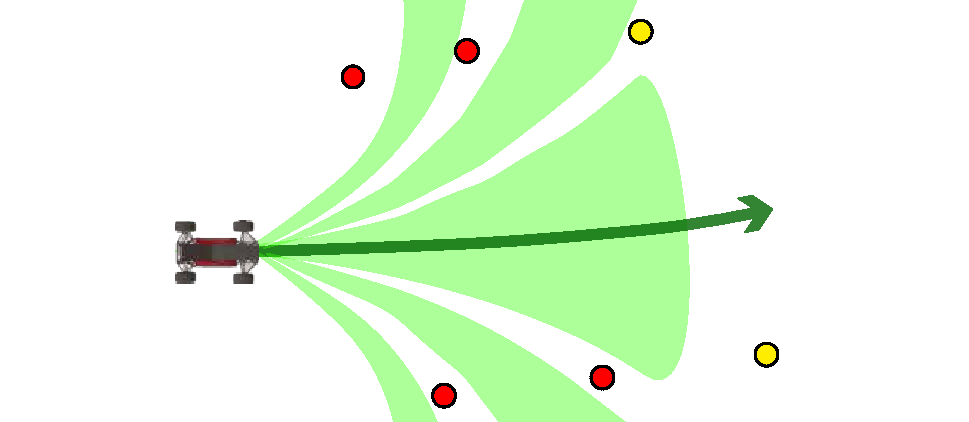
\includegraphics[width=0.9\linewidth]{conedriving}
	\caption[Visualisation of the path planner on cone driving]{Visualisation of the path planner on cone driving. Immediate cones are red and subsequent cones are yellow; green regions are viable paths. }
	\label{fig:7:conedrive}
\end{figure}

Paths are generated through the clustering and filtering of LiDAR data. With reference to Fig.~\ref{fig:7:conedrive}, the vehicle will drive straight following the green arrow in the green region as it has the largest range free of objects. Path planning for cone driving was tested across three sets of recordings $N$ to verify the consistency of path generation across all subsequent frames $\Sigma n$. Frames with false positives and negatives are considered erroneous frames $n_e$, where the error percentage $e$ is then calculated with our results given as Table~\ref{tbl:7:frame}. With a mean false detection of less than 5\% and the erroneous frames at less than 8\%. We have therefore deduced from these results that our cone driving algorithm is adequate for autonomous driving. Note that these errors can be further remedied with frame coherence, which is capable of eliminating the classification of stray frames.

\begin{table}[H]
	\caption{Path Errors}
	\label{tbl:7:frame}
	\centering
	\begin{tabular}{cccc}
		\toprule
		$N$ & $n_e$ & $\Sigma n$ &  $e$   \\ \midrule
		 1  &   7   &     84     & 7.14\% \\
		 2  &   3   &     62     & 4.84\% \\
		 3  &   1   &     24     & 4.17\% \\ \bottomrule
	\end{tabular}
\end{table}

The runtime performances of individual nodes were recorded during our experiments, which are given in percentages as their means and standard deviations for CPU (avgCPU, stdCPU) and memory consumption (avgRAM, stdRAM), as tabulated in Table~\ref{tbl:7:runtime}. The sensors’ driver nodes make up the largest utilisation percentage, with the image captures occupying over 60\% of the CPU footprint to capture a series of 3-channel, 8-bit calibrated RGB image from the camera pair. The LiDARs collectively consume 18\% of CPU. The path planning (ConeDetect) and high-level control nodes operate at 20 Hz, with 11\% CPU usage.

\nomenclature[z-cpu]{CPU}{Central processing unit}

\begin{table}[H]
	\caption{Runtime Performances for Cone Driving}
	\label{tbl:7:runtime}
	\centering
	\begin{tabular}{lrrrr}
		\toprule
		Nodes      &  avgCPU  &  stdCPU  & avgRAM & stdRAM  \\ \midrule
		Camera     & 63.47\%  & 3.862\%  & 1.5\%  &  0.0\%  \\
		IMU        & 7.157\%  & 0.5182\% & 1.9\%  &  0.0\%  \\
		LUX        & 9.955\%  & 0.6802\% & 1.7\%  &  0.0\%  \\
		LMS111     & 7.586\%  & 0.4830\% & 0.30\% &  0.0\%  \\
		ConeDetect & 7.605\%  & 0.7858\% & 0.38\% & 0.040\% \\
		roscore    & 0.1354\% & 0.1909\% & 0.88\% & 0.61\%  \\
		control    & 3.557\%  & 0.2461\% & 0.30\% &  0.0\%  \\ \bottomrule
	\end{tabular}
\end{table}

\subsection{Driving Simulation}\label{sec:7:benchdrive}
The effectiveness of the simulation system was measured through the drawing of comparisons to results gathered from testing of the SAE vehicle. Given the current work involving autonomously driving a traffic cone delineated race track, a focus was placed on the relative accuracy of the LiDAR and visual cone detection systems compared to results gained from test drives of the SAE vehicle. Comparisons were made by recreating a cone track on a flat plane in the simulation system and performing visual comparisons of the results. A comparison of the tracks used is displayed in Fig.~\ref{fig:7:scenarioComparison}.

\begin{figure}[H]
	\centering
	\begin{subfigure}[b]{0.45\textwidth}
		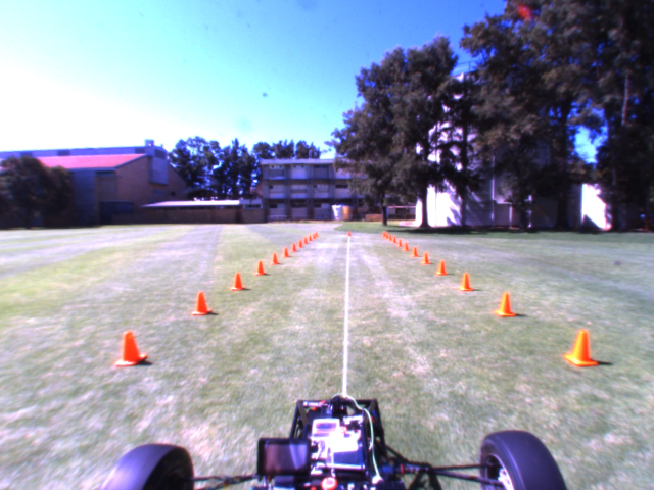
\includegraphics[width=\textwidth]{scenario-real}
		\caption{Real}
		\label{fig:7:sc:real}   
	\end{subfigure} 
	\hspace{1em}         
	\begin{subfigure}[b]{0.45\textwidth}
		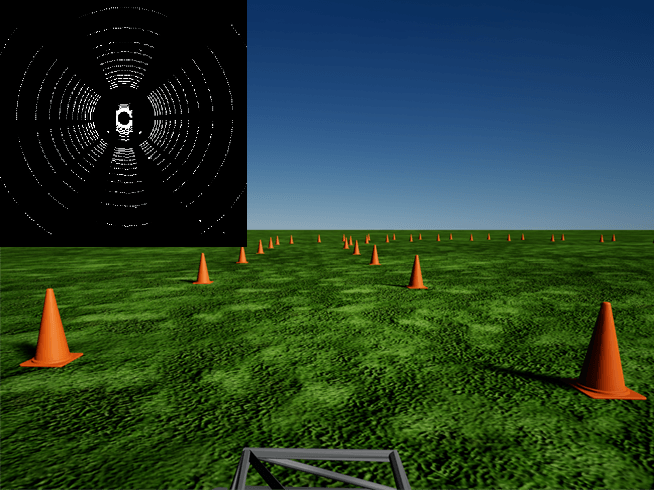
\includegraphics[width=\textwidth]{scenario-sim}
		\caption{Simulated}
		\label{fig:7:sc:sim}
	\end{subfigure}             
	\caption[Real and simulated LiDAR scenarios for visual cone processing]{Scenarios used for comparing (a) real and (b) simulated LiDAR and visual cone processing outputs.}
	\label{fig:7:scenarioComparison}
\end{figure}

From Fig.~\ref{fig:7:lidarComparison}, the output from the simulated LiDAR is significantly more detailed than that on the SAE vehicle. As such, the original LiDAR output from the simulator (white points) was cropped to simulate the LiDAR available on the SAE vehicle through the use of ROS' ``pointcloud\_to\_laserscan'' package, resulting in the 2D laser scan data displayed in green. While these laser scans are not identical, with the real data displaying the ground on the far right as a result, of the uneven terrain, these figures show that the cone locations identified are sufficiently similar to allow testing of higher level components (e.g. path planning) on the simulated system.

\begin{figure}[H]
	\centering
	\begin{subfigure}[b]{0.45\textwidth}
		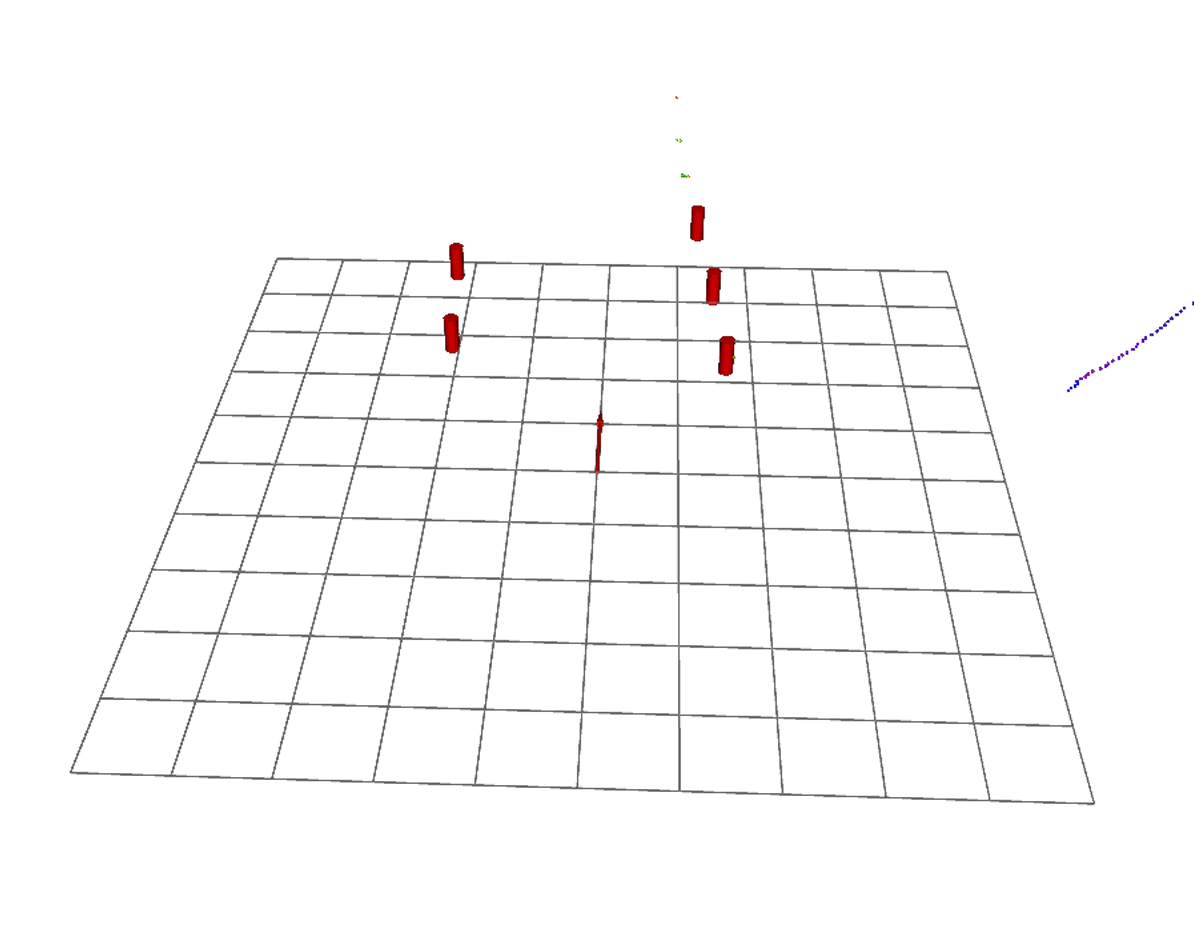
\includegraphics[width=\textwidth]{lidar-real}
		\caption{Real}
		\label{fig:7:lidarComparison:1}   
	\end{subfigure} 
	\hspace{1em}         
	\begin{subfigure}[b]{0.45\textwidth}
		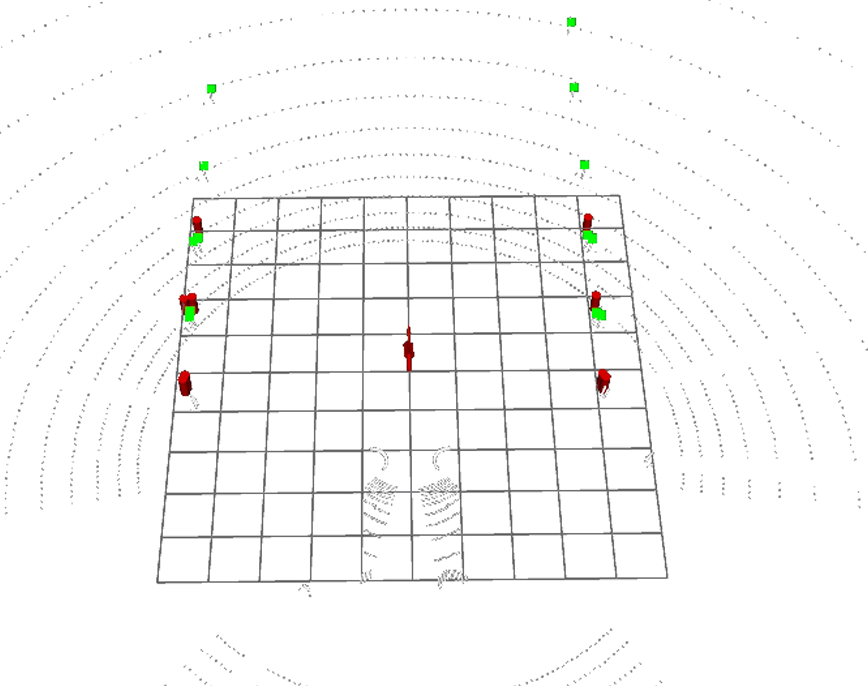
\includegraphics[width=\textwidth]{lidar-sim}
		\caption{Simulated}
		\label{fig:7:lidarComparison:2}
	\end{subfigure}             
	\caption[Real and simulated LiDAR output for visual cone processing]{LiDAR cone processing outputs from (a) real and (b) simulated scenarios.}
	\label{fig:7:lidarComparison}
\end{figure}

\section{Conclusion}\label{sec:7:conclusion}
We have presented a software framework for a high-level control system that is designed for autonomous vehicles that is both modular and scalable. Our design approach using open-source software with commercially available sensors and parts hopes to encourage similar projects especially in academia where we have fitted a student competition vehicle for full autonomous driving. These projects can therefore be low-cost while allowing users to adapt the software to the vehicle's and environment's needs. This system aims to be holistic by incorporating all the necessary modules required for autonomous driving, including sensor interfaces and fusion, localisation, path planning, visual navigation and road detection; as well as cone driving and an identical driving simulator for both real-world and simulated tests.  It is therefore easily deployable while requiring minimal configuration. Experiments on path planning, cone driving and the simulator proved that this system is robust and adequate for implementation. We are eager to correspond with any entities who wish to incorporate our approach in their respective projects. 